\chapter{Le CAR-T: Nuovi approcci terapeutici al linfoma non-Hodgkin}

\section{Introduzione alle CAR-T}

La terapia cellulare con CAR-T (Chimeric Antigen Receptor) è una forma di terapia genica impiegata per forme 
refrattarie e recidivanti  i cui risultati più importanti si hanno per la leucemia linfoblastica acuta e per il 
linfoma non Hodgkin (LNH). Sono in corso ricerche che consentano l’impiego di tale metodica anche per altre neoplasie 
ematologiche nonché per i tumori solidi.\\
La terapia delle CAR-T è autologa, in quanto usa le cellule T proprie del paziente. La loro produzione sfrutta 
il processo di ingegnerizzazione. Il CAR è un recettore transmembrana chimerico, che, mediante l’utilizzo di 
vettori retrovirali o lentivirali, va a sostituire il TCR del linfocita.\\
L’European Medicines Agency (EMA) ha dato l’approvazione commerciale di due CAR-T di seconda generazione: 
tisagenlecleucel (tisa-cel, KymriahTM, Novartis) e axicabtagene ciloleucel (axi-cel, YescartaTM, Gilead), 
che sono anche i prodotti disponibili in Italia\cite{reteveneta}.\\
Nel caso del LNH, Tisagenlecleucel è indicato per i linfomi diffusi a grandi cellule B (DLBCL) recidivanti o 
refrattari dopo due linee di chemioterapia sistemica.\\ Axicabtageneciloleucel è stato approvato per linfomi 
diffusi a grandi cellule B (DLBCL) e linfoma a grandi cellule B primitivo del mediastino, 
refrattari o recidivanti, dopo due linee di chemioterapia sistemica\cite{EMATOCART}.\\
La FDA (Food and Drugs Administration) ha invece approvato sei farmaci (Figura \ref{fig:FIGURE_3.8}), come 
riportato dal National Cancer Institute\cite{NIHCART}.\\

\begin{figure}[H]
    \begin{center}
    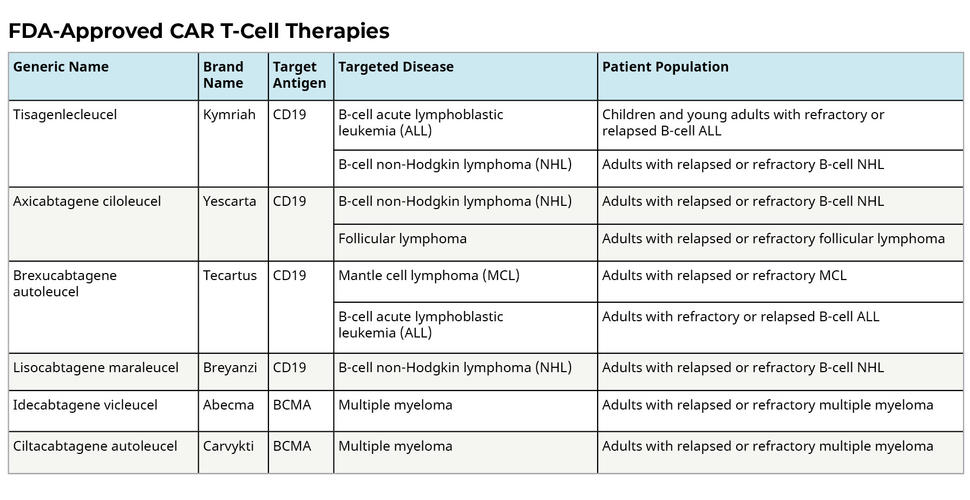
\includegraphics[width=1.0\columnwidth]{img/FDAApprovedCART.jpeg}
    \end{center}
    \caption{Farmaci CAR-T approvati dall’FDA
    \cite{NIHCART}}
    \label{fig:FIGURE_3.8}
\end{figure}

\section{Fasi del processo di costituzione delle CAR-T}

La prima fase del processo di produzione delle CAR-T è la leucoaferesi, in cui viene prelevato il sangue dal 
paziente tramite una vena periferica; grazie al processo di aferesi il sangue prelevato viene separato in 
globuli rossi, globuli bianchi, piastrine e plasma, ma solo le cellule T dei globuli bianchi vengono prelevate, 
mentre il resto del sangue viene reinfuso al paziente.\\
È una fase molto importante e delicata in quanto una bassa resa aferetica, provoca una 
ridotta espansione delle cellule CAR-T in vitro; questo può dipendere da una bassa conta leucocitaria, 
dalla presenza di numerose cellule natural killer (NK) e blasti nel sangue periferico\cite{EMATOCART},\cite{LLSCART}.\\

La seconda fase del processo prevede che le cellule T raccolte siano inviate a laboratori specializzati per la fase 
di ingegnerizzazione genetica, secondo cui il DNA viene introdotto all’interno delle cellule, per produrre CAR, 
grazie ai quali le cellule T acquisiscono la capacità di attaccare le cellule cancerose\cite{EMATOCART},\cite{LLSCART}.\\

Nella terza fase, il numero di cellule raccolte viene moltiplicato in laboratorio e quando si ha il quantitativo 
necessario, vengono criopreservate e rinviate al centro o all’ospedale dove il paziente le riceverà. 
Questo processo dura dalle tre alle quattro settimane.\\
Prima della somministrazione, il paziente, a partire da una settimana fino a due giorni prima, viene sottoposto 
alla chemioterapia di linfodeplezione che  serve a ridurre le cellule T normali nel corpo, per “fare spazio” alle 
cellule CAR-T ed avere una maggiore espansione in vivo.\\ 
Lo schema terapeutico maggiormente utilizzato prevede la somministrazione di ciclofosfamide e fludarabina.\\

L’ultima fase è di somministrazione del farmaco, previo scongelamento, in una via endovenosa centrale, 
della durata di circa trenta minuti\cite{EMATOCART}.\\
I centri autorizzati alla somministrazione delle CAR-T sono presenti in tutta Italia, in Toscana abbiamo 
i centri di Firenze e Pisa\cite{AILCENTRI}.\\

\begin{figure}[H]
    \begin{center}
    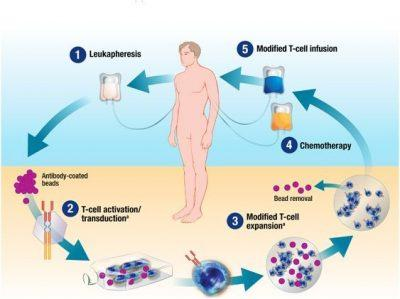
\includegraphics[width=0.58\columnwidth]{img/car-tprocess.jpeg}
    \end{center}
    \caption{Processo di costituzione e somministrazione delle CAR-T
    \cite{EMATOCART}}

\end{figure}

\begin{figure}[H]
    \begin{center}
    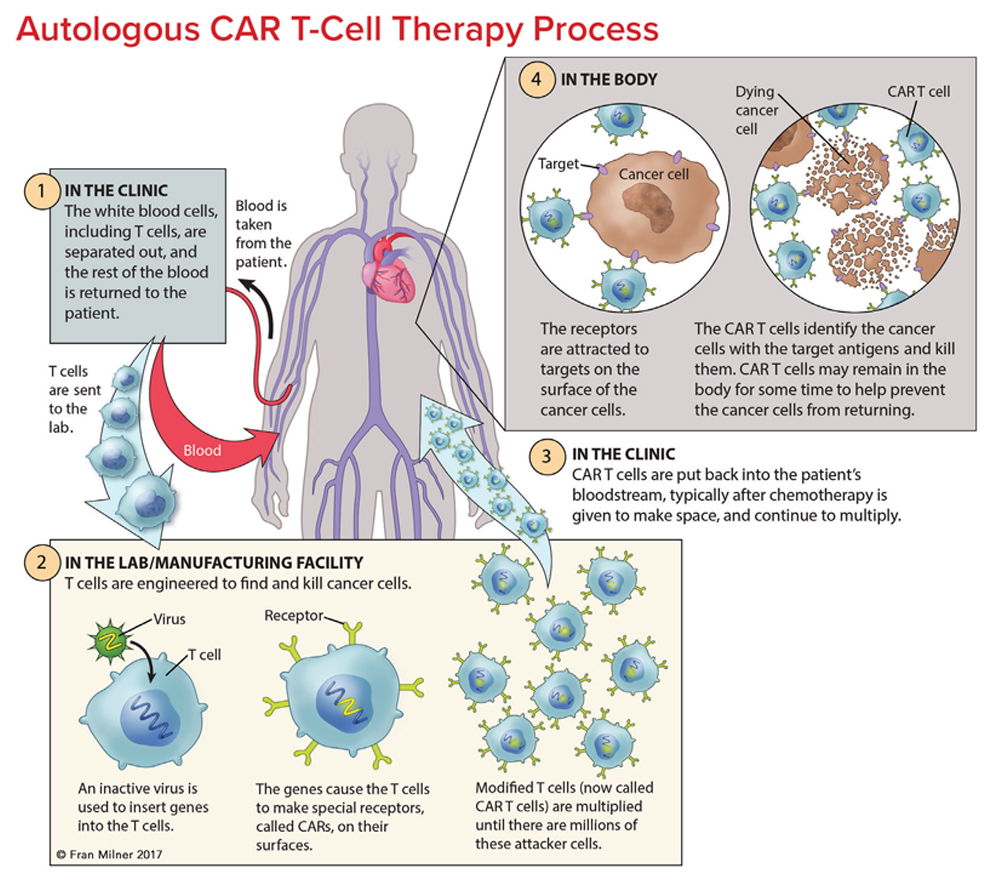
\includegraphics[width=0.8\columnwidth]{img/CART-TherapyProcess.jpeg}
    \end{center}
    \caption{Processo di prelievo, costituzione e somministrazione delle CAR-T
    \cite{LLSCART}}

\end{figure}

\section{Complicanze correlate al processo di somministrazione delle CAR-T}

Nonostante i risultati positivi dati dalla terapia delle CAR-T, che dimostrano il raggiungimento di risposte rapide e 
durature nel tempo, non mancano aspetti di tossicità acuta, che possono evolvere in situazioni di severità, se non 
anche di fatalità\cite{EMATOCART}.\\

\subsection{Sindrome da rilascio di citochine (CRS)}

Più frequentemente si assiste ad una sindrome da rilascio di citochine (CRS), che può manifestarsi con sintomi come 
astenia, febbre, mal di testa, tachicardia, ipotensione e ipossia, sintomi sistemici quali arresto cardiaco, aritmia, 
encefalopatia, insufficienza renale, fino ad arrivare ad una insufficienza multiorgano. La CRS può inoltre evolvere 
in una MAS (sindrome da attivazione macrofagica). 
La CRS può insorgere a partire da alcune ore, fino anche ad una settimana dalla somministrazione di CAR-T.\\
Diversi sono i fattori di rischio che comportano il manifestarsi di tale sintomatologia (Figura \ref{fig:FIGURE_3.11}) che 
influiscono anche sul suo grado di severità; ad esempio un’ infusione di una dose elevata di CAR-T, le caratteristiche 
del paziente, il tipo di terapia di linfodeplezione, lo stato della malattia e il  burden di malattia 
(burden of disease), che dà una stima dell’impatto della malattia in termini di disabilità e mortalità\cite{EMATOCART}.\\

\begin{figure}[H]
    \begin{center}
    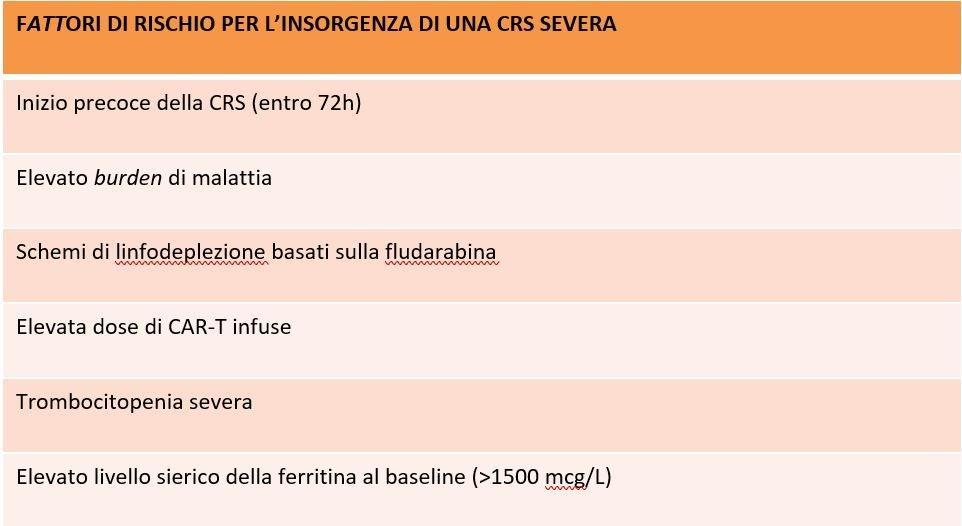
\includegraphics[width=0.7\columnwidth]{img/rischioCRS.jpeg}
    \end{center}
    \caption{Fattori di rischio per l’insorgenza di una CRS severa. 
    \cite{EMATOCART}}
    \label{fig:FIGURE_3.11}
\end{figure}

Il grado di severità con cui si sviluppa la CRS è correlato agli elevati livelli ematici di CAR-T ed elevati livelli 
sierici di IL-6 (interleuchina-6); pertanto il trattamento di prima scelta della CRS moderata-severa, 
prevede la somministrazione di tocilizumab, un anticorpo monoclonale anti-IL-6\cite{EMATOCART}.\\
L’uso di corticosteroidi per la CRS, era precedentemente limitato, ma secondo studi più recenti il loro utilizzo 
non compromette l'attività delle CAR-T e l’outcome del paziente\cite{Cortico}.\\
Per valutare il grado di severità della CRS, l’ASTCT (American Society for Transplantation and Cellular Therapy) 
ha prodotto delle linee guida\cite{ASTCT}.\\

\begin{figure}[H]
    \begin{center}
    \includegraphics[width=0.8\columnwidth]{img/severitàCRS.jpeg}
    \end{center}
    \caption{Criteri di valutazione del grado di severità CRS.
    \cite{EMATOCART}}

\end{figure}

\subsection{Immune effector cell-associated neurotoxicity syndrome (ICANS)}

La neurotossicità è un effetto collaterale comune alla terapia con CAR-T. 
L’ASTCT (American Society for Transplantation and Cellular Therapy) ha definito la neurotossicità con 
l’acronimo ICANS (Immune effector cell-associated neurotoxicity syndrome). Non sono ancora del tutto chiare le 
motivazioni per cui tale sintomatologia si presenta, sono in corso studi che cercano di spiegare i meccanismi 
fisiopatologici coinvolti.\\
L’ ICANS si manifesta con afasia, disturbi dell’attenzione, difficoltà alla scrittura, confusione, disorientamento, 
agitazione, tremori e sonnolenza. In caso di ICANS severa, i sintomi che possono presentarsi sono: crisi convulsive, 
edema cerebrale, aumento della pressione intracranica,, incontinenza, deficit di forza\cite{EMATOCART}.\\
L’ ICANS può presentarsi in concomitanza della CRS, in tal caso ha una minore durata e severità; può insorgere anche 
in seguito alla CRS con maggiore durata e severità. La durata dei sintomi è variabile, in genere è di circa 2-4 giorni,
ma può durare anche diverse settimane; i sintomi sono solitamente reversibili. 
Il trattamento terapeutico con tocilizumab è efficace in caso di ICANS associata a CRS, altrimenti la terapia di 
elezione è con corticosteroidi\cite{EMATOCART}.\\
L’ ASTCT (American Society for Transplantation and Cellular Therapy) 
ha prodotto anche per ICANS delle linee guida per valutare il grado di severità\cite{ASTCT}.\\

\begin{figure}[H]
    \begin{center}
    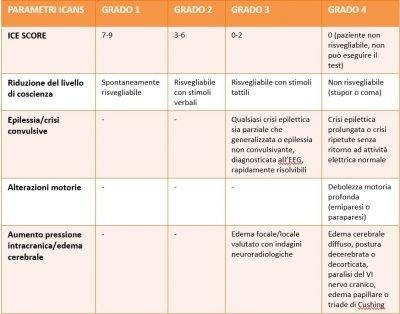
\includegraphics[width=0.7\columnwidth]{img/ICANS.jpeg}
    \end{center}
    \caption{Parametri per la valutazione del grado di severità di ICANS.
    \cite{EMATOCART}}

\end{figure}

\subsection{Sindrome da Attivazione Macrofagica (MAS)}

Nella sindrome da attivazione macrofagica (MAS), si ha un’iperattività di macrofagi e linfociti, che stimolano la 
produzione di citochine pro-infiammatorie, che creano degli infiltrati tissutali, con rischio di insorgenza di 
insufficienza multiorgano.\\
I sintomi di CRS e MAS sono simili: febbre, sintomatologia neurologica, insufficienza multiorgano; 
per quanto riguarda gli esami laboratoristici si avranno livelli elevati di LDH, ferritina e citochine, mentre 
ridotti livelli di fibrinogeno\cite{EMATOCART}.
Nei pazienti in cui si sospetta una MAS, con tossicità d’organo >3, si intraprende terapia con anticorpi monoclonali 
anti-IL-6 e corticosteroidi, in caso di non miglioramento entro 48 ore, 
si prende in considerazione la terapia con etoposide.\\
La MAS refrattaria e fulminante si presenta nell’1\% circa dei pazienti trattati con CAR-T, 
se non trattata prontamente ha un’elevata mortalità\cite{EMATOCART}.\\

\subsection{Altre reazioni avverse}

La tossicità autoimmune si verifica quando il linfocita CAR-T riconosce come antigene target il CD-19 non solo nelle 
cellule cancerose, ma anche nelle cellule sane.
Il fenomeno è noto come “on-target-of-tissue effects”. È un effetto avverso che può risultare anche fatale.
È ciò che succede ai linfociti B sani, che presentano sulla loro superficie il target del linfocita CAR-T e vanno 
incontro ad aplasia. La ricerca, dovrebbe orientarsi a trovare una soluzione affinchè il target delle cellule CAR-T 
siano le cellule cancerose e non quelle sane\cite{Frontiers}.\\

Una reazione anafilattica si può verificare per reazione eccessiva del sistema immunitario nei confronti del CAR, 
pertanto bisogna monitorare la comparsa di eventuali segni e sintomi come eritemi, 
sudorazione, ipotensione e distress respiratorio\cite{EMATOCART}.
Nel caso in cui si evidenzia la comparsa di tali sintomi, il trattamento viene sospeso o terminato\cite{Frontiers}.\\

Le infezioni associate alla somministrazione di CAR-T (CTI), sono piuttosto comuni. Non è del tutto noto il meccanismo 
che le innesca e non c’è uno schema unico per la loro prevenzione e trattamento. Vi sono tuttavia una serie di fattori 
che possono indurre tali infezioni: i pazienti molto spesso sviluppano come effetto avverso alla terapia delle CAR-T 
una CRS, che può portare al ricovero del paziente in unità di terapia intensiva, dove aumenta il rischio di sviluppare 
infezioni nosocomiali; il trattamento con farmaci corticosteroidi per la CRS indebolisce il sistema immunitario, che a  
sua volta, risulta indebolito anche dalla riduzione di cellule B sane, che sono il target del CD-19 delle CAR-T; 
i pazienti che hanno un indebolimento del sistema immunitario causato dalla chemioterapia e che poi ricevono le CAR-T, 
sono ad elevato rischio di sviluppare infezioni\cite{Frontiers}.\\

La Tumor Lysis Syndrome (TLS) è una complicanza abbastanza comune, maggiormente nelle neoplasie ematologiche piuttosto 
che nelle altre.\\ 
Si verifica perché un elevato numero di cellule cancerose diventano necrotiche e rilasciano i loro metaboliti e le 
loro sostanze intracellulari nel sangue; i reni non riescono ad eliminare completamente queste sostanze ed è per 
questo che si verifica la TLS.\\ 
Segni di TLS sono iperpotassiemia, iperuricemia, iperfosfatemia e ipocalcemia, in casi gravi insufficienza renale 
acuta e aritmia.\\ 
Il trattamento prevede l’ idratazione; per pazienti con rischio da basso a moderato si può intraprendere la 
somministrazione di allopurinolo in via preventiva; il rasburicase è il trattamento di elezione sia per prevenzione 
di pazienti ad alto rischio che per pazienti che hanno già sviluppato una TLS; somministrazione di diuretici e 
correzione degli squilibri idroelettrolitici\cite{Frontiers}.\\

Disturbi della coagulazione a volte si presentano, tra i 6 e i 20 giorni dopo l’infusione di CAR-T. Ci sarà un  
aumento del D-dimero, il PT allungato, trombocitopenia, diminuzione del fibrinogeno. Il rischio di CID 
(coagulazione intravascolare disseminata) è maggiore in pazienti con CRS grave, 
che risulta essere direttamente proporzionale alla gravità dei disturbi della coagulazione\cite{Frontiers}.\\

La citopenia è una reazione avversa caratterizzata da neutropenia, trombocitopenia ed anemia. 
È stato dimostrato che la citopenia che insorge in seguito alla somministrazione di CAR-T può avere una durata anche 
superiore a 30 giorni\cite{Frontiers}.\\ 
Pazienti con citopenia lieve e precoce devono avere un supporto nutrizionale e intraprendere dei trattamenti di 
prevenzione anti-infettiva.\\ 
Per pazienti con neutropenia a lungo termine, la FDA ha approvato la somministrazione mediante iniezione di Filgrastim. 
Pazienti con anemia e trombocitopenia grave vengono sottoposti a trasfusione di sangue, globuli rossi e piastrine. 
È stato anche proposto il trapianto autologo o allogenico di cellule staminali emopoietiche, come trattamento per 
la citopenia, ma la sua efficacia non è ancora ben nota\cite{Frontiers}.\\

\section{L’infermiere e le CAR-T}

Le CAR-T sono una nuova strategia di trattamento per il linfoma di non Hodgkin, nuovi studi sono orientati verso 
l’utilizzo di questa terapia anche per stadi iniziali della patologia. È doveroso sottolineare il ruolo centrale 
che gli infermieri hanno verso l’impiego delle CAR-T, dalla preparazione del paziente, prelievo delle cellule del 
paziente stesso, infusione delle CAR-T costituite, alla post-infusione, ed anche nel follow-up del paziente. 
Tuttavia non mancano gli effetti collaterali e le tossicità, di seria importanza\cite{NURSINGCART}.\\
La diffusione, sempre più ampia, della terapia delle CAR-T, sta determinando il cambiamento del ruolo e delle 
responsabilità infermieristiche. Questa terapia, prevede per il paziente, un approccio multidisciplinare, che vada a 
combinarsi con i bisogni e le difficoltà cliniche, sociali e finanziarie, della cura al paziente. Il ruolo degli 
infermieri pertanto è fondamentale, dal punto di vista della sorveglianza clinica, coordinazione delle cure ed 
educazione al paziente, non senza difficoltà, perché queste terapie richiedono nuovi bisogni, di cui gli infermieri 
possono non avere esperienza a riguardo. Le strutture ospedaliere che eseguono queste procedure di trattamento, 
devono assicurare aggiornamento e formazione infermieristica, riguardo la gestione di questa 
tipologia di paziente e di approccio terapeutico\cite{article2}.\\
 
Il paziente oncoematologico che riceve il trattamento CAR-T, è molto complesso, agli infermieri è richiesto, 
di agire, con l’abilità di riconoscere, monitorare e classificare eventuali tossicità nel 
percorso del paziente; essi svolgono un ruolo chiave nell’educazione del paziente, nella coordinazione, 
nel trattamento\cite{NURSINGCART}.\\
Il fatto che, ad oggi, le CAR-T, siano un’opzione di trattamento per stati di malattia relativamente avanzati o comunque 
per forme recidive/refrattarie che non hanno risposto ad altri trattamenti (standard o terapie sperimentali), 
genera sentimenti d’ansia, i pazienti possono soffrire di isolamento sociale, soprattutto se sono in cura in centri 
lontani dalla loro sede e di conseguenza dalle persone significative. Tutto il team multidisciplinare deve essere a 
conoscenza di questi fattori; il nursing prevede di assicurarsi che il paziente, i familiari e la figura del caregiver, 
ricevano le giuste informazioni che riguardano test, procedure, istruzioni sulla gestione dell’accesso 
venoso centrale e le potenziali complicanze che ne potrebbero derivare\cite{NURSINGCART}.\\

Quando il paziente è candidato a ricevere la terapia CAR-T, l’infermiere deve accertarsi che il paziente abbia eseguito 
tutti i test necessari, per quanto riguarda la valutazione della funzionalità epatica, 
renale, cardiaca, polmonare, per garantire sicurezza al trattamento\cite{article2}. Prima dell’infusione, 
bisogna effettuare i test necessari, per ridurre il rischio di complicanze che potrebbero derivare 
da infezioni batteriche, virali e fungine\cite{NURSINGCART}.\\
Si valuta, per una bridging chemotherapy, basata sul principio secondo cui, pazienti la cui malattia è particolarmente 
aggressiva, da potersi espandere, se non trattata nel periodo di tempo di attesa della ricostituzione delle CAR-T, 
potrebbero necessitare di chemioterapia. Bisogna valutare il “burden of disease” del paziente, cioè l’impatto che 
la malattia ha in termini di disabilità e mortalità. 
In caso di bisogno di chemioterapia, bisogna considerare comunque gli eventuali rischi associati (TLS, CRS)\cite{article3}.\\

Per la somministrazione di CAR-T, gli infermieri devono tenere conto di una serie di passaggi: identificare il paziente e 
illustrare la procedura, verificare la presenza del consenso informato firmato in cartella, controllare la correttezza 
della prescrizione, rilevare i parametri vitali, assicurando che il paziente sia apiretico ed emodinamicamente stabile, 
documentare in cartella, controllare l’accesso venoso; predisporre nelle vicinanze del paziente, il carrello delle 
emergenze, verificando che tutto il materiale sia presenze e i dispositivi funzionanti. Somministrare eventuale 
pre-medicazione se prevista, iniziare l’infusione usando i set di infusione che arrivano con le cellule, monitorare 
la comparsa di eventuali reazioni correlate all’infusione. Paziente e caregiver devono essere informati in forma 
verbale e scritta, riguardo possibili reazioni avverse, la necessità di riferire eventuali sintomi e rimanere 
nelle vicinanze dell’ospedale per almeno 4 settimane dopo la terapia, 
il paziente deve evitare di guidare per 8 settimane dopo l’infusione\cite{NURSINGCART}.\\

Indipendentemente dallo svolgimento del trattamento in regime ambulatoriale o di ricovero ordinario, 
il ruolo dell’infermiere durante l’infusione del prodotto resta imperativo; essi devono essere adeguatamente 
formati e pronti, riguardo la gestione di  effetti avversi che possono verificarsi durante l’infusione, 
già al momento della presa in carico del paziente\cite{article2}.\\
Il riconoscimento e la classificazione precoce, possono aiutare gli infermieri oncologici, nella selezione di interventi 
basati sulle evidenze, che possano permettere la gestione e l’annullamento di effetti collaterali potenzialmente 
minacciosi per la vita stessa del paziente. Agli infermieri, si consiglia di adottare nella pratica clinica, 
metodi di classificazione e valutazione oggettivi, come parte dell’agire quotidiano, soprattutto nei 
casi in cui si sospettano complicanze come la neurotossicità, i cui cambiamenti possono insorgere 
rapidamente nel tempo\cite{article4}.\\

Parte del management infermieristico prevede oltre alla valutazione del paziente, anche l’accertamento da parte 
dell’infermiere della presenza di tutti i mezzi di supporto necessari al paziente durante il trattamento. 
Ad esempio alcuni centri di cura, richiedono al paziente di restare ad una specifica distanza dal centro stesso, 
fino a 30 giorni dopo l’infusione di CAR-T, per consentire l’accesso del paziente alla struttura, in tempi ragionevoli, 
nel caso insorgessero complicanze o effetti avversi dopo la dimissione. Il consulto infermieristico da effettuare 
prima dell’approvazione del paziente per il trattamento, bisogna assicurarsi sulla presenza del caregiver, 
poiché le istituzioni si muovono sempre di più verso una scelta ambulatoriale per l’esecuzione di tali procedure, 
per ridurre i costi e i ricoveri in ospedale, per cui il ruolo del caregiver si dimostra di cruciale importanza. 
Questa esigenza, si traduce nel bisogno di educare il caregiver, nel riconoscimento precoce di segni e sintomi delle 
principali complicanze correlate all’infusione delle CAR-T, nonché sull’importanza di riferire eventuali potenziali 
effetti avversi al team sanitario. Come riportato dall’autore, senza un caregiver adatto a rispondere ai 
bisogni del paziente in modo appropriato, il paziente potrebbe non essere un candidato ottimale 
alla terapia delle CAR-T\cite{article2}.\\

Vista la crescita nell’uso delle CAR-T, la ONS (Oncology Nursing Society), ha sviluppato una risorsa, 
proprio con lo scopo di migliorare l’apprendimento dei meccanismi correlati ai vari processi che costituiscono 
le CAR-T, gli effetti avversi potenzialmente più comuni e le considerazioni infermieristiche su come trattarli\cite{ONSCART}.\\

\begin{figure}[H]
    \begin{center}
    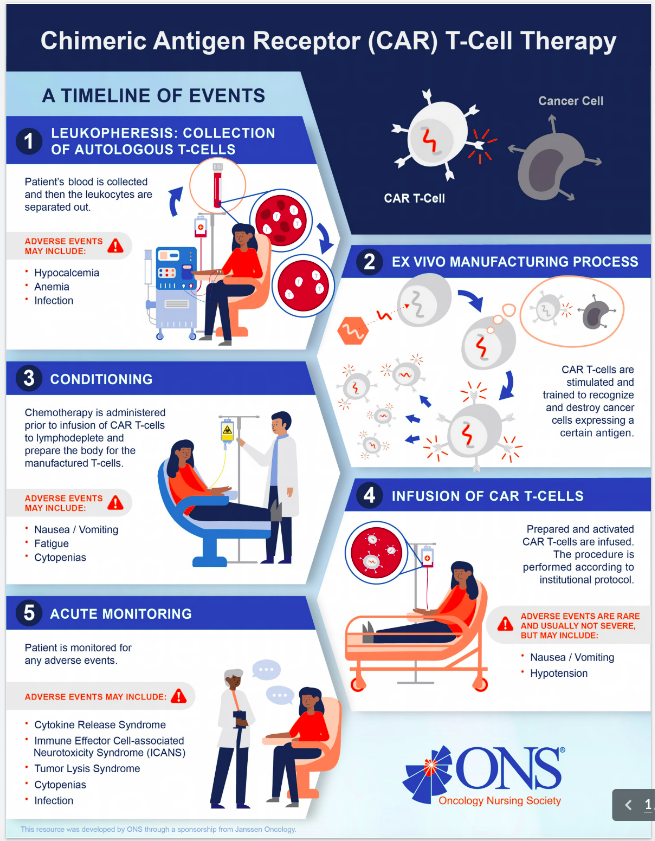
\includegraphics[width=0.9\columnwidth]{img/CAR-T-PROCESS.png}
    \end{center}
    \caption{Fasi del processo CAR-T.
    \cite{ONSCART}}

\end{figure}

\begin{figure}[H]
    \begin{center}
    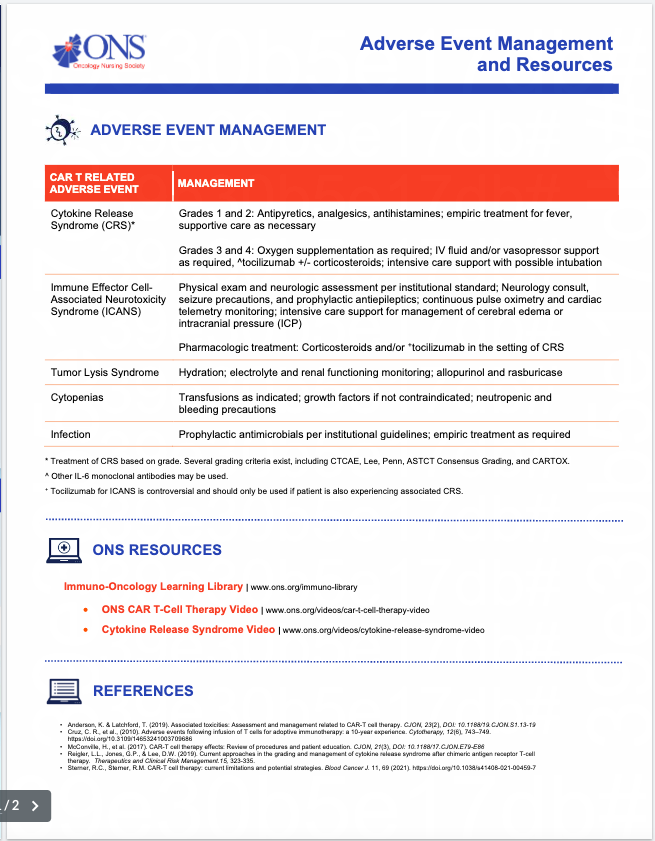
\includegraphics[width=0.9\columnwidth]{img/CAR-T-SIDE-EFFECTS.png}
    \end{center}
    \caption{Complicanze della terapia CAR-T e gestione.
    \cite{ONSCART}}

\end{figure}


\section{Il dolore nel paziente oncologico}

Il dolore è considerato il quinto parametro vitale ed è uno dei sintomi che più preoccupa il paziente, 
in quanto impatta negativamente sulla qualità di vita.\\ La gestione del dolore, 
è una delle dimensioni di cura più importanti, il ruolo degli infermieri è fondamentale, 
dal punto di vista sia della valutazione, sia per quanto riguarda il trattamento farmacologico e non farmacologico.\\ 
Dallo studio condotto, gli infermieri, non hanno abbastanza conoscenze a riguardo (sono stati riportati risultati 
medio-bassi); essi pertanto devono essere adeguatamente formati, dal momento che all’interno del team di 
assistenza sono le figure più importanti coinvolte con i pazienti oncologici\cite{PAIN}.\\
Il dolore è un’esperienza multidimensionale, che coinvolge la sfera biologica, psicologica, sociale, ed è 
influenzata da fattori ambientali; può essere di tipo acuto, cronico, refrattario, e i pazienti possono 
provare tutti questi tipi di dolore insieme, per cui diventa difficile comprendere l’esperienza provata dal 
paziente.\\ Secondo le stime  della WHO, più del 90\% del dolore oncologico può essere controllato, 
con interventi di routine. Nonostante siano molti gli interventi da poter attuare seguendo le evidenze, 
i pazienti continuano a soffrire, perché le pratiche non vengono applicate quotidianamente.
\cite{PAINONS}.\\

Il dolore del paziente oncologico, dipende dal tipo di neoplasia, dalle terapie antineoplastiche, 
dalla presenza di comorbilità. È fondamentale valutare il dolore e monitorare il paziente sull’andamento 
del dolore dopo aver messo in atto degli interventi. Bisogna valutare il dolore per quanto riguarda: 
localizzazione (i pazienti possono riferire di avere dolore anche in più di un punto, talvolta chiedere di 
localizzarlo può aiutare a capirne la causa), che tipo di dolore è (neuropatico, somatico o viscerale), 
da quanto tempo è insorto e se è continuo o intermittente, intensità (da valutare utilizzando le scale 
di valutazione del dolore), qual è il piano terapeutico attuale per il controllo del dolore e la risposta 
del paziente ad esso; considerare che il dolore di tipo refrattario, nel 10-20\% dei pazienti, 
non risponde all’analgesia standard\cite{CANCERPAINONS}.\\
Le problematiche di dipendenza/abuso di oppioidi, possono interferire con l’ottimale gestione del dolore oncologico. 
Spesso, per paura di instaurare problematiche di dipendenza, si evita la prescrizione di tali farmaci, 
ma in questo modo il dolore non viene gestito e i pazienti continuano a soffrire; 
è una questione che rappresenta un dilemma per medici e infermieri, per cui occorre un’attenta valutazione\cite{PAINONS}.\\ 
Vi sono evidenze che dimostrano che è possibile somministrare oppioidi per il controllo del dolore nei pazienti con SUDs 
(substance use disorders), fondamentale è la prevenzione delle ricadute. Riconoscere le ricadute può essere difficile, 
questi pazienti tendono a nasconderlo, per cui bisogna programmare un percorso di detossificazione graduale, 
da non vedere come un fallimento, ma come parte del processo di guarigione\cite{CANCERPAINONS}.\\

Secondo la ONS, la responsabilità degli infermieri e dei medici, nei confronti del paziente e dei familiari, 
è di agire applicando le EBP (evidence based practice); la ONS riconosce tuttavia che la ricerca 
può risultare difficoltosa, motivo per cui si impegna a fornire agli infermieri 
evidenze e raccomandazioni per la pratica clinica\cite{PAINONS}.\\

\section{La comunicazione tra infermiere e paziente}

L’infermiere deve essere consapevole del suo ruolo professionale, deve agire con competenza e preparazione e se non 
sufficientemente preparato è obbligato a formarsi ed aggiornarsi.\\ 
L’infermiere è colui che stabilisce una relazione di aiuto costante e prolungata con il paziente oncologico e i suoi 
familiari, fornisce supporto psicologico ed emotivo, deve promuovere il ruolo del caregiver e del nucleo familiare; 
deve aiutare il paziente nel processo di accettazione dei cambiamenti che intervengono nella sua vita a causa della 
malattia, cambiamenti che ricopriranno un lungo periodo, a causa sia della malattia, che del presidio venoso di cui 
avrà bisogno, che avrà lo scopo di facilitare il programma di cura, ma con possibili complicanze; l’infermiere però 
deve anche riuscire a sviluppare nel paziente una capacità di autocura e autogestione della malattia, orientandolo 
verso l’autonomia.\\
L’infermiere oltre a sapere e saper fare, deve saper essere, ovvero possedere quelle capacità comunicative e 
relazionali, insieme ad empatia e umanità, che sono proprie della sua figura; deve promuovere nella persona la 
consapevolezza della malattia e la conoscenza del percorso clinico-assistenziale, sostenendo la persona nella 
scelta del trattamento più adatto\cite{COMUNICAZIONE}.\\
Il supporto al paziente viene dato mediante l’educazione del paziente stesso, circa lo stile di vita, la dieta, la 
estione delle complicanze, la descrizione di procedure diagnostico-terapeutiche, il controllo e gestione dei sintomi. 
Il bisogno emotivo del paziente si traduce in un bisogno di informazioni, di rassicurazione, vicinanza emotiva, 
empatia, pertanto l’infermiere deve essere preparato ad accogliere la sofferenza del paziente e dei suoi familiari.\\
I pazienti molto spesso avvertono un profondo senso di solitudine, causato dall’impossibilità di comunicare con i 
loro cari, con le persone significative, non riescono ad occupare le giornate in modo da essere soddisfatti, questo 
perchè talvolta sono sottoposti a ricoveri in regime di isolamento, oppure in unità operative ad accesso controllato 
(come la terapia intensiva), hanno bisogno di assistenza per le attività pratiche e questo può provocare 
nel paziente profondo disagio.\\
Si parla di comunicazione terapeutica quando si entra in sintonia con l’altro ed egli riesce a chiedere aiuto e a 
sentirsi ascoltato, compreso, accettato e non giudicato\cite{NURSE24}.\\
Il processo di assistenza infermieristica comprenderà l'identificazione dei problemi infermieristici, del paziente e 
della famiglia, la pianificazione di interventi, l’implementazione di un piano di assistenza sulla base degli 
obiettivi prefissati, la valutazione dei risultati ottenuti.\\
